\section{Tecnicas Básicas de Compressão}

\begin{frame}%[allowframebreaks]
  \frametitle{Leitura}
  \centering
  
\includegraphics[width=0.4\textwidth]{images/qrcode-book-salomon.pdf}

  David Salomon, Giovanni Motta - \textit{Handbook of Data Compression}, 2010 \\ 
  \url{https://books.google.com.br/books?id=LHCY4VbiFqAC}\\
  Introduction, Basic Techniques \citep{salomon2010}
\end{frame} 

\subsection{RLE}
\begin{frame}%[allowframebreaks]
  \frametitle{Compressão RLE}
   
  Exemplo:

  string: `2. all is too well'

  codificação: `2. a@2l is t@2o we@2l'

  \vspace{1cm}
  Método MNP5 era utilizado nos modems antigos.

\end{frame}
\note{
MNP : Microcom Networking Protocol

"The MNP5 method is a two-stage process that starts with run-length encoding, followed by adaptive frequency encoding."
\citep{salomon2000}

"With MNP 5, the data received from the computer are first compressed with a simple algorithm, and then passed into the MNP 4 packetizing system for transmission. On best-case data the system offered about 2:1 compression, but in general terms about 1.6:1 was typical, at least on text. As a result a 2400 bit/s modem would appear to transfer text at ~4000 bit/s, even though the modem was still running at the same 600 baud * 4 bits per symbol rate.

This dramatic increase in throughput allowed Microcom modems to remain somewhat competitive with models from other companies that were otherwise nominally much faster. For instance, Microcom generally produced 1200 and 2400 bit/s modems using commodity parts, while companies like USRobotics and Telebit offered models with speeds up to 19200 bit/s."
(\url{https://en.wikipedia.org/wiki/Microcom_Networking_Protocol})
}


\begin{frame}%[allowframebreaks]
  \frametitle{Compressão RLE}
 
  Exemplo: uma imagem em tons de cinza com 8-bit de profundidade começa com os seguintes valores

  12, 12, 12, 12, 12, 12, 12, 12, 12, 35, 76, 112, 67, 87, 87, 87, 5, 5, 5, 5, 5, 5, 1, ...

  será comprimida como  \framebox{9},12,35,76,112,67,\framebox{3},87,\framebox{6},5,1, ...

  \vspace{1cm}
  Se utilizarmos como \textit{flag} o valor 255, então a sequência acima será expressa por

  255, 9, 12, 35, 76, 112, 67, 255, 3, 87, 255, 6, 5, 1, ...

  \vspace{1cm}
  grupos de 8

  \framebox{10000010},9,12,35,76,112,67,3,87,\framebox{100...},6,5,1, ...

\end{frame} 

\begin{frame}%[allowframebreaks]
  \frametitle{Exemplo RLE - GNU Octave}
  \centering
  
\includegraphics[width=0.4\textwidth]{images/qrcode-jupyter-rle.pdf}

  \url{https://nbviewer.jupyter.org/github/leolca/notebooks/blob/master/aev/rle_mario.ipynb}
\end{frame} 


\begin{frame}%[allowframebreaks]
  \frametitle{Move-to-Front Coding}
  Consideramos o alfabeto de símbolos $\mathcal{A}$ como uma lista 
  onde os símbolos mais frequentes estarão dispostos no início da lista.

  O método é localmente adaptativo, já que ele se adapta à frequência dos
  símbolos em cada região do fluxo de dados.
\end{frame} 


\begin{frame}%[allowframebreaks]
  \frametitle{Move-to-Front Coding - Exemplo \citep{salomon2010}}

   Exemplo:
   entrada a ser codificada: \textbf{abcddcbamnopponm}

  \begin{columns}[c]
  \column{.4\textwidth}
  C = (0, 1, 2, 3, 0, 1, 2, 3, 4, 5, 6, 7, 0, 1, 2, 3) \\
  -- utilizando move-to-front\\
  \vspace{1cm}
  C' = (0, 1, 2, 3, 3, 2, 1, 0, 4, 5, 6, 7, 7, 6, 5, 4) \\
  -- sem utilizar move-to-front 
  \column{.6\textwidth}
     \vspace{-0.2cm}
     \begin{figure}[h!]
     \centering
     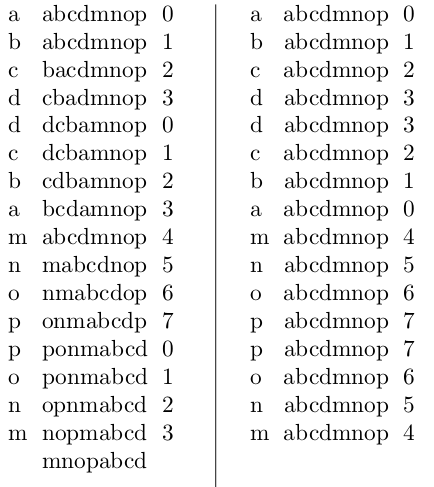
\includegraphics[width=0.7\textwidth]{images/move_to_front_coding.png}
     %\caption{}
     \label{fig:move_to_front_coding}
     \end{figure}
  \end{columns}

\end{frame} 

\begin{frame}%[allowframebreaks]
  \frametitle{Move-to-Front Coding - Exemplo \citep{salomon2010}}
  \begin{columns}[c]
  \column{.4\textwidth}
  O resultado $C$ obtido pelo move-to-front é tal que, na média, os valores
  em $C$ são pequenos (os valores no início do dicionário são os mais prováveis).
  Isto faz com que a saída seja propícia para ser codificada através da codificação
  de Huffman ou codificação aritmética.
  \column{.4\textwidth}
     \begin{figure}[h!]
     \centering
     \includegraphics[width=0.65\textwidth]{/home/leoca/ee/ufsj/2012_01/audio_video/aulas/images/variable_sized_codes.png}
     \caption{Exemplo de código de tamanho variável.}
     \label{fig:variable_sized_codes}
     \end{figure}
  \end{columns}

\end{frame}


\begin{frame}%[allowframebreaks]
  \frametitle{Move-to-Front Coding}
  Variações:
  \begin{enumerate}
  \item Move-ahead-k: O elemento do alfabeto A que corresponde ao símbolo corrente será deslocado k posições para cima na lista ao
          invés de ir para o topo da lista.
  \item Wait-c-and-move: O elemento do alfabeto A será deslocado para o início da lista apenas após aparecer c vezes durante a
          codificação. 
  item Wait-c-and-ahead-k: Um combinação das duas variantes anteriores.
  \end{enumerate}

\end{frame} 

\begin{frame}%[allowframebreaks]
  \frametitle{Exemplo Move-to-Front - GNU Octave}
  \centering
  
\includegraphics[width=0.4\textwidth]{images/qrcode-jupyter-m2f.pdf}

  \url{https://nbviewer.jupyter.org/github/leolca/notebooks/blob/master/aev/move-to-front.ipynb}
\end{frame} 




